%%%%%%%%%%%%%%%%%%%%%%%%%%%%%%%%%%%%%%%%%
% a0poster Portrait Poster
% LaTeX Template
% Version 1.0 (22/06/13)
%
% The a0poster class was created by:
% Gerlinde Kettl and Matthias Weiser (tex@kettl.de)
% 
% This template has been downloaded from:
% http://www.LaTeXTemplates.com
%
% License:
% CC BY-NC-SA 3.0 (http://creativecommons.org/licenses/by-nc-sa/3.0/)
%
%%%%%%%%%%%%%%%%%%%%%%%%%%%%%%%%%%%%%%%%%

%----------------------------------------------------------------------------------------
%   PACKAGES AND OTHER DOCUMENT CONFIGURATIONS
%----------------------------------------------------------------------------------------

\documentclass[a0,portrait]{a0poster}

\usepackage{multicol} % This is so we can have multiple columns of text side-by-side
\columnsep=100pt % This is the amount of white space between the columns in the poster
\columnseprule=0pt % This is the thickness of the black line between the columns in the poster

\usepackage[svgnames]{xcolor} % Specify colors by their 'svgnames', for a full list of all colors available see here: http://www.latextemplates.com/svgnames-colors

\usepackage{times} % Use the times font
%\usepackage{palatino} % Uncomment to use the Palatino font

\usepackage{graphicx} % Required for including images
\graphicspath{{figures/}} % Location of the graphics files
\usepackage{booktabs} % Top and bottom rules for table
\usepackage[font=small,labelfont=bf]{caption} % Required for specifying captions to tables and figures
\usepackage{amsfonts, amsmath, amsthm, amssymb} % For math fonts, symbols and environments
\usepackage{wrapfig} % Allows wrapping text around tables and figures

\begin{document}

%----------------------------------------------------------------------------------------
%   POSTER HEADER 
%----------------------------------------------------------------------------------------

% The header is divided into two boxes:
% The first is 75% wide and houses the title, subtitle, names, university/organization and contact information
% The second is 25% wide and houses a logo for your university/organization or a photo of you
% The widths of these boxes can be easily edited to accommodate your content as you see fit
\begin{center}
{\veryHuge \color{NavyBlue} \textbf{Modelling of cardiac cross-bridge
cycling during ischemia}\\ [2cm]}% Title
\end{center}
%\Huge\textit{An Exploration of Complexity}\\[2cm] % Subtitle
\begin{minipage}[b]{0.63\linewidth}
\huge \textbf{Mario Uhrin$\mathbf{^1}$, \underline{Andrej
    Klic$\mathbf{^1}$} and Ivan Valent$\mathbf{^2}$}\\[0.4cm] % Author(s)
\Large $\mathbf{^1~}$Department of Pharmacology and Toxicology, Faculty of Pharmacy\\
Comenius University, Bratislava, Slovakia \\[0.2cm]
\Large $\mathbf{^2~}$Department of Physical and Theoretical Chemistry, Faculty of Nat.~Sciences\\
Comenius University, Bratislava, Slovakia\\[0.2cm]
\Large Contact:~\texttt{klic1@uniba.sk}\\
\end{minipage}
%
\begin{minipage}[b]{0.45\linewidth}

\includegraphics[scale=0.30]{faf-prif_logos}\\
\end{minipage}

\vspace{2cm} % A bit of extra whitespace between the header and poster content

%----------------------------------------------------------------------------------------

\begin{multicols}{2} % This is how many columns your poster will be broken into, a portrait poster is generally split into 2 columns

%%----------------------------------------------------------------------------------------
%%   ABSTRACT
%%----------------------------------------------------------------------------------------
%
%\color{Navy} % Navy color for the abstract
%
%\begin{abstract}
%
%Sed fringilla tempus hendrerit. Vestibulum ante ipsum primis in faucibus orci luctus et ultrices posuere cubilia Curae; Etiam ut elit sit amet metus lobortis consequat sit amet in libero. Lorem ipsum dolor sit amet, consectetur adipiscing elit. Phasellus vel sem magna. Nunc at convallis urna. isus ante. Pellentesque condimentum dui. Etiam sagittis purus non tellus tempor volutpat. Donec et dui non massa tristique adipiscing. Quisque vestibulum eros eu. Phasellus imperdiet, tortor vitae congue bibendum, felis enim sagittis lorem, et volutpat ante orci sagittis mi. Morbi rutrum laoreet semper. Morbi accumsan enim nec tortor consectetur non commodo nisi sollicitudin. Proin sollicitudin. Pellentesque eget orci eros. Fusce ultricies, tellus et pellentesque fringilla, ante massa luctus libero, quis tristique purus urna nec nibh.
%
%\end{abstract}

%----------------------------------------------------------------------------------------
%   INTRODUCTION
%----------------------------------------------------------------------------------------

\color{SaddleBrown} % SaddleBrown color for the introduction

\section*{Introduction}

In sudden oxygen delivery cut-off, the metabolical changes occurs, which
have direct impact on cycle of heart muscle contraction. The
concentrations of ATP and creatine-phosphate are quickly decreasing and
cummulation of ADP, phospates and protons occurs. The cell metabolism
decreases and switches to anaerobic regime. Ions like calcium and sodium
are cummulating in cell, which can lead as far as to infarct, the
apoptosis. 

Our work discusses the contractile cyrcle (crossbridge), affected by
metabolites acummulating during oxygen deficiency, the ischemia.
Metabolites like phosphates and protons are acummulating during ischemia
and are directly interferring with the crossbridge cycle, which
manifestates as decrease in myocardial contractile force.

%----------------------------------------------------------------------------------------
%   OBJECTIVES
%----------------------------------------------------------------------------------------

\color{DarkSlateGray} % DarkSlateGray color for the rest of the content

\section*{Theory}

\begin{center}\vspace{0.5cm}
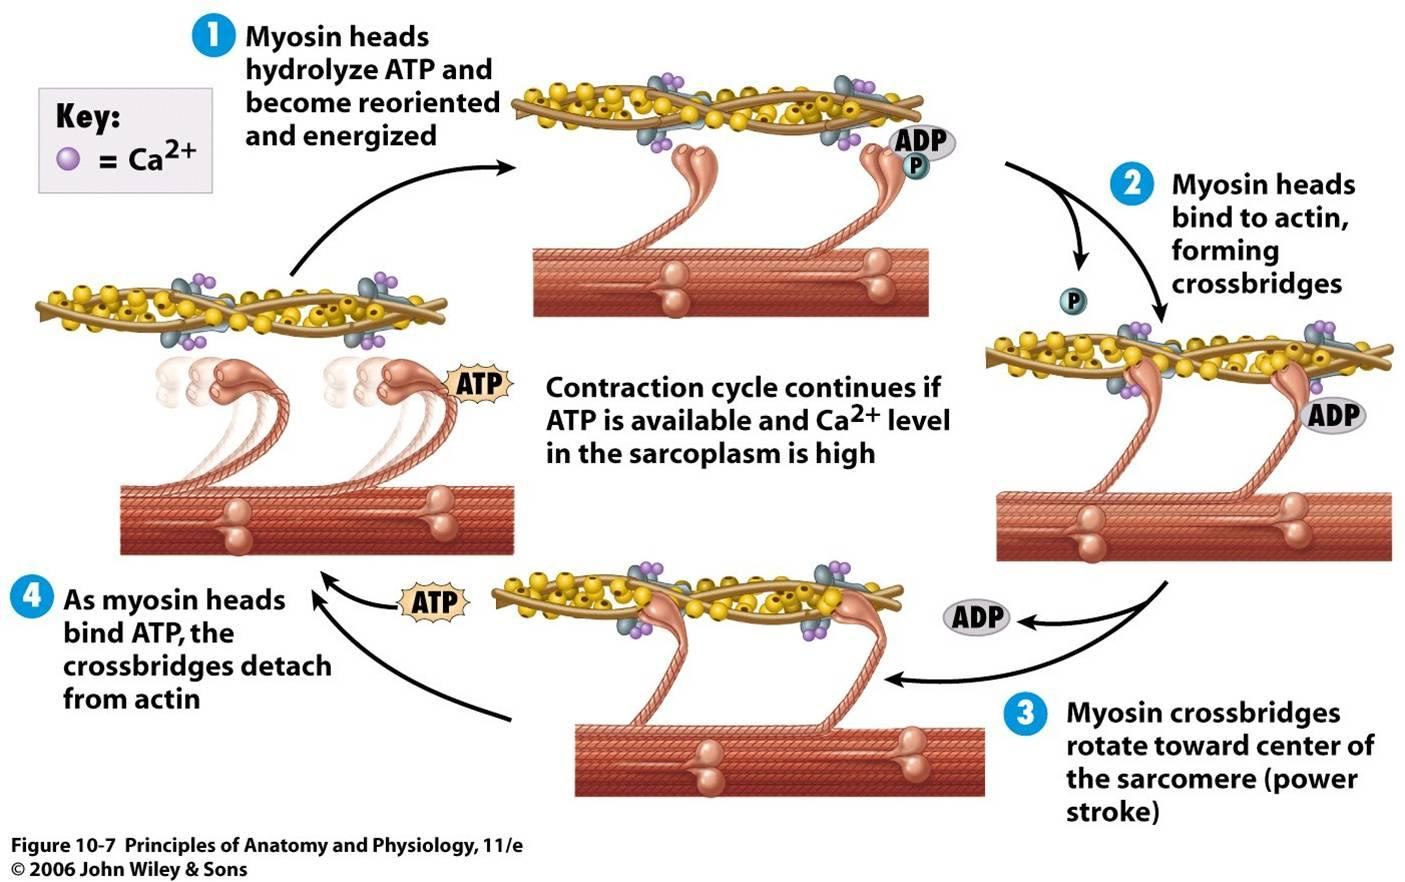
\includegraphics[scale=0.5]{muscle-contraction_hi-res}
\captionof{figure}{\color{Green} Figure caption}
\end{center}%\vspace{1cm}

%\section*{Main Objectives}
%
%\begin{enumerate}
%\item Lorem ipsum dolor sit amet, consectetur.
%\item Nullam at mi nisl. Vestibulum est purus, ultricies cursus volutpat sit amet, vestibulum eu.
%\item Praesent tortor libero, vulputate quis elementum a, iaculis.
%\item Phasellus a quam mauris, non varius mauris. Fusce tristique, enim tempor varius porta, elit purus commodo velit, pretium mattis ligula nisl nec ante.
%\item Ut adipiscing accumsan sapien, sit amet pretium.
%\item Estibulum est purus, ultricies cursus volutpat
%\item Nullam at mi nisl. Vestibulum est purus, ultricies cursus volutpat sit amet, vestibulum eu.
%\item Praesent tortor libero, vulputate quis elementum a, iaculis.
%\end{enumerate}



%----------------------------------------------------------------------------------------
%   Methods and Implementation
%----------------------------------------------------------------------------------------

\section*{Methods and Implementation}

Base model [Tran, 2010], implemented in CellML was exported as Python
code. Our model is using the the mean-field approximations implemented as
set of ODEs. The numerical analysis was performed using VODE integrator
with BDF method from the Python SciPy package. Resulting data were
visualised with the ggplot2 plotting system supplied in R programming
language distribution.

\begin{center}%\vspace{1cm}
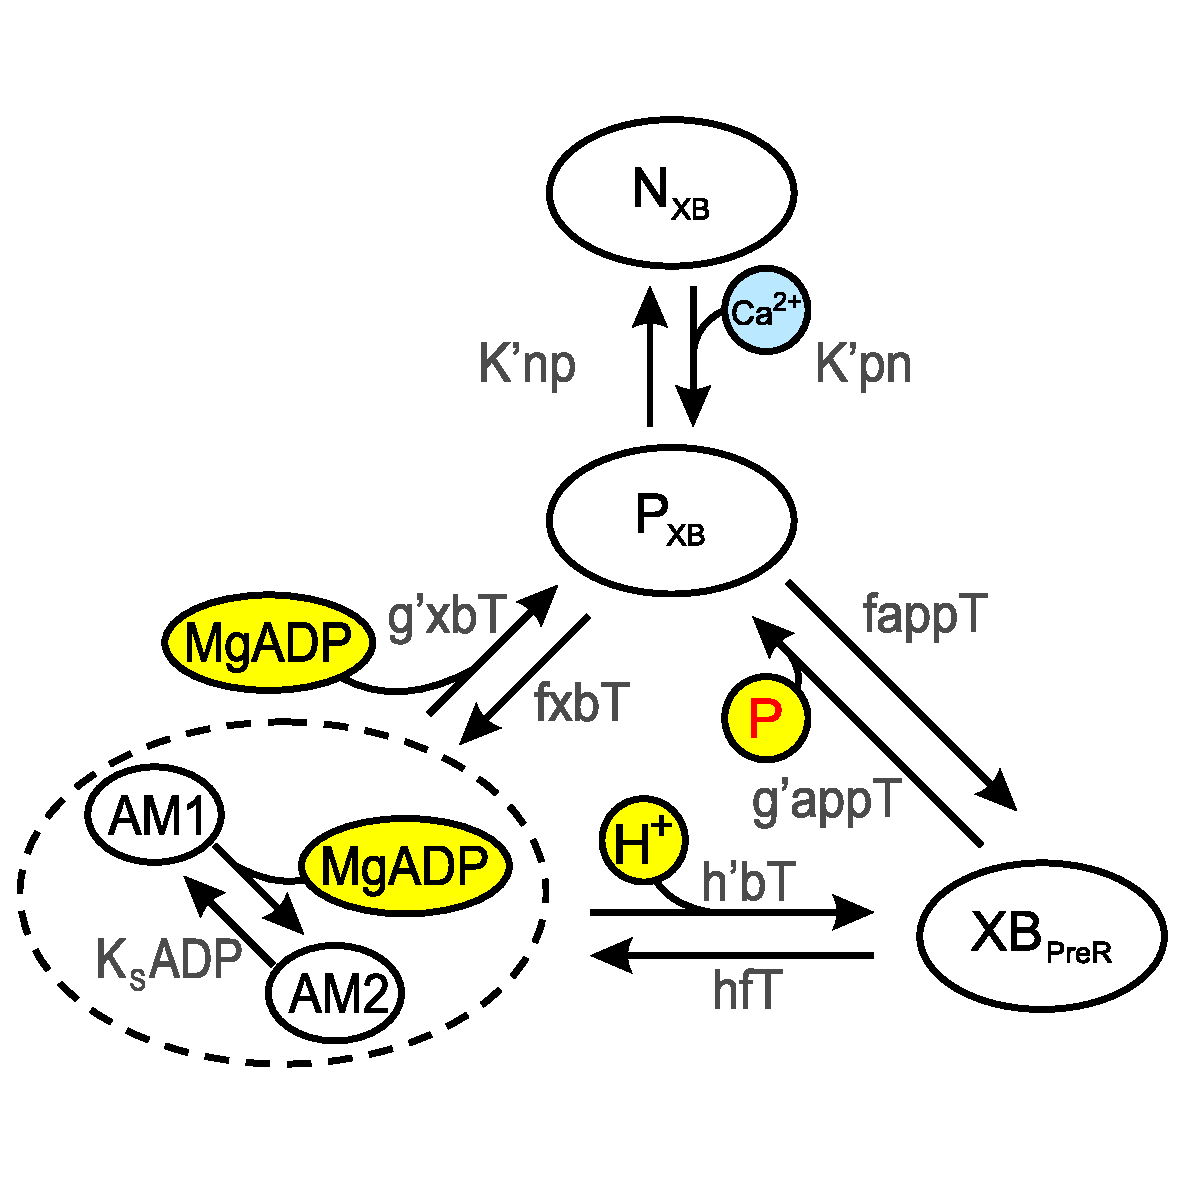
\includegraphics[scale=0.7]{cross-bridge_scheme_v2}
\captionof{figure}{\color{Green} Figure caption}
\end{center}%\vspace{1cm}

%------------------------------------------------

%\subsection*{Mathematical Section}

%Nulla vel nisl sed mauris auctor mollis non sed. 

%\begin{eqnarray}
%\cos\bar{\phi}_k Q_{j,k+1,t} + Q_{j,k+1,x}+\frac{\sin^2\bar{\phi}_k}{T\cos\bar{\phi}_k} Q_{j,k+1} &=&\nonumber\\ 
%-\cos\phi_k Q_{j,k,t} + Q_{j,k,x}-\frac{\sin^2\phi_k}{T\cos\phi_k} Q_{j,k}\label{edgek}
%\end{eqnarray}
%and
%\begin{eqnarray}
%\cos\bar{\phi}_j Q_{j+1,k,t} + Q_{j+1,k,y}+\frac{\sin^2\bar{\phi}_j}{T\cos\bar{\phi}_j} Q_{j+1,k}&=&\nonumber \\
%-\cos\phi_j Q_{j,k,t} + Q_{j,k,y}-\frac{\sin^2\phi_j}{T\cos\phi_j} Q_{j,k}.\label{edgej}
%\end{eqnarray} 
%
%Nulla sed arcu arcu. Duis et ante gravida orci venenatis tincidunt. Fusce
%vitae lacinia metus. Pellentesque habitant morbi.
%$\mathbf{A}\underline{\xi}=\underline{\beta}$ Vim $\underline{\xi}$ enum
%nidi $3(P+2)^{2}$ lacina. Id feugain $\mathbf{A}$ nun quis; magno.

%----------------------------------------------------------------------------------------
%   RESULTS 
%----------------------------------------------------------------------------------------

\section*{Results}

Donec faucibus purus at tortor egestas eu fermentum dolor facilisis.
Maecenas tempor dui eu neque fringilla rutrum. Mauris \emph{lobortis} nisl
accumsan. Aenean vitae risus ante.
%
%\begin{wraptable}{l}{12cm} % Left or right alignment is specified in the
%first bracket, the width of the table is in the second \begin{tabular}{l
%l l} \toprule \textbf{Treatments} & \textbf{Response 1} &
%\textbf{Response 2}\\ \midrule Treatment 1 & 0.0003262 & 0.562 \\
%Treatment 2 & 0.0015681 & 0.910 \\ Treatment 3 & 0.0009271 & 0.296 \\
%\bottomrule \end{tabular} \captionof{table}{\color{Green} Table caption}
%\end{wraptable}
%
Phasellus imperdiet, tortor vitae congue bibendum, felis enim sagittis
lorem, et volutpat ante orci sagittis mi. Morbi rutrum laoreet semper.
Morbi accumsan enim nec tortor consectetur non commodo nisi sollicitudin.
Proin sollicitudin. Pellentesque eget orci eros. Fusce ultricies, tellus
et pellentesque fringilla, ante massa luctus libero, quis tristique purus
urna nec nibh.

Nulla ut porttitor enim. Suspendisse venenatis dui eget eros gravida
tempor. Mauris feugiat elit et augue placerat ultrices. Morbi accumsan
enim nec tortor consectetur non commodo. Pellentesque condimentum dui.
Etiam sagittis purus non tellus tempor volutpat. Donec et dui non massa
tristique adipiscing. Quisque vestibulum eros eu. Phasellus imperdiet,
tortor vitae congue bibendum, felis enim sagittis lorem, et volutpat ante
orci sagittis mi. Morbi rutrum laoreet semper. Morbi accumsan enim nec
tortor consectetur non commodo nisi sollicitudin.

%\begin{center}\vspace{1cm}
%\includegraphics[width=0.8\linewidth]{placeholder}
%\captionof{figure}{\color{Green} Figure caption}
%\end{center}\vspace{1cm}

%In hac habitasse platea dictumst. Etiam placerat, risus ac.
%
%Adipiscing lectus in magna blandit:
%
%\begin{center}\vspace{1cm}
%\begin{tabular}{l l l l}
%\toprule
%\textbf{Treatments} & \textbf{Response 1} & \textbf{Response 2} \\
%\midrule
%Treatment 1 & 0.0003262 & 0.562 \\
%Treatment 2 & 0.0015681 & 0.910 \\
%Treatment 3 & 0.0009271 & 0.296 \\
%\bottomrule
%\end{tabular}
%\captionof{table}{\color{Green} Table caption}
%\end{center}\vspace{1cm}

\begin{center}%\vspace{1cm}
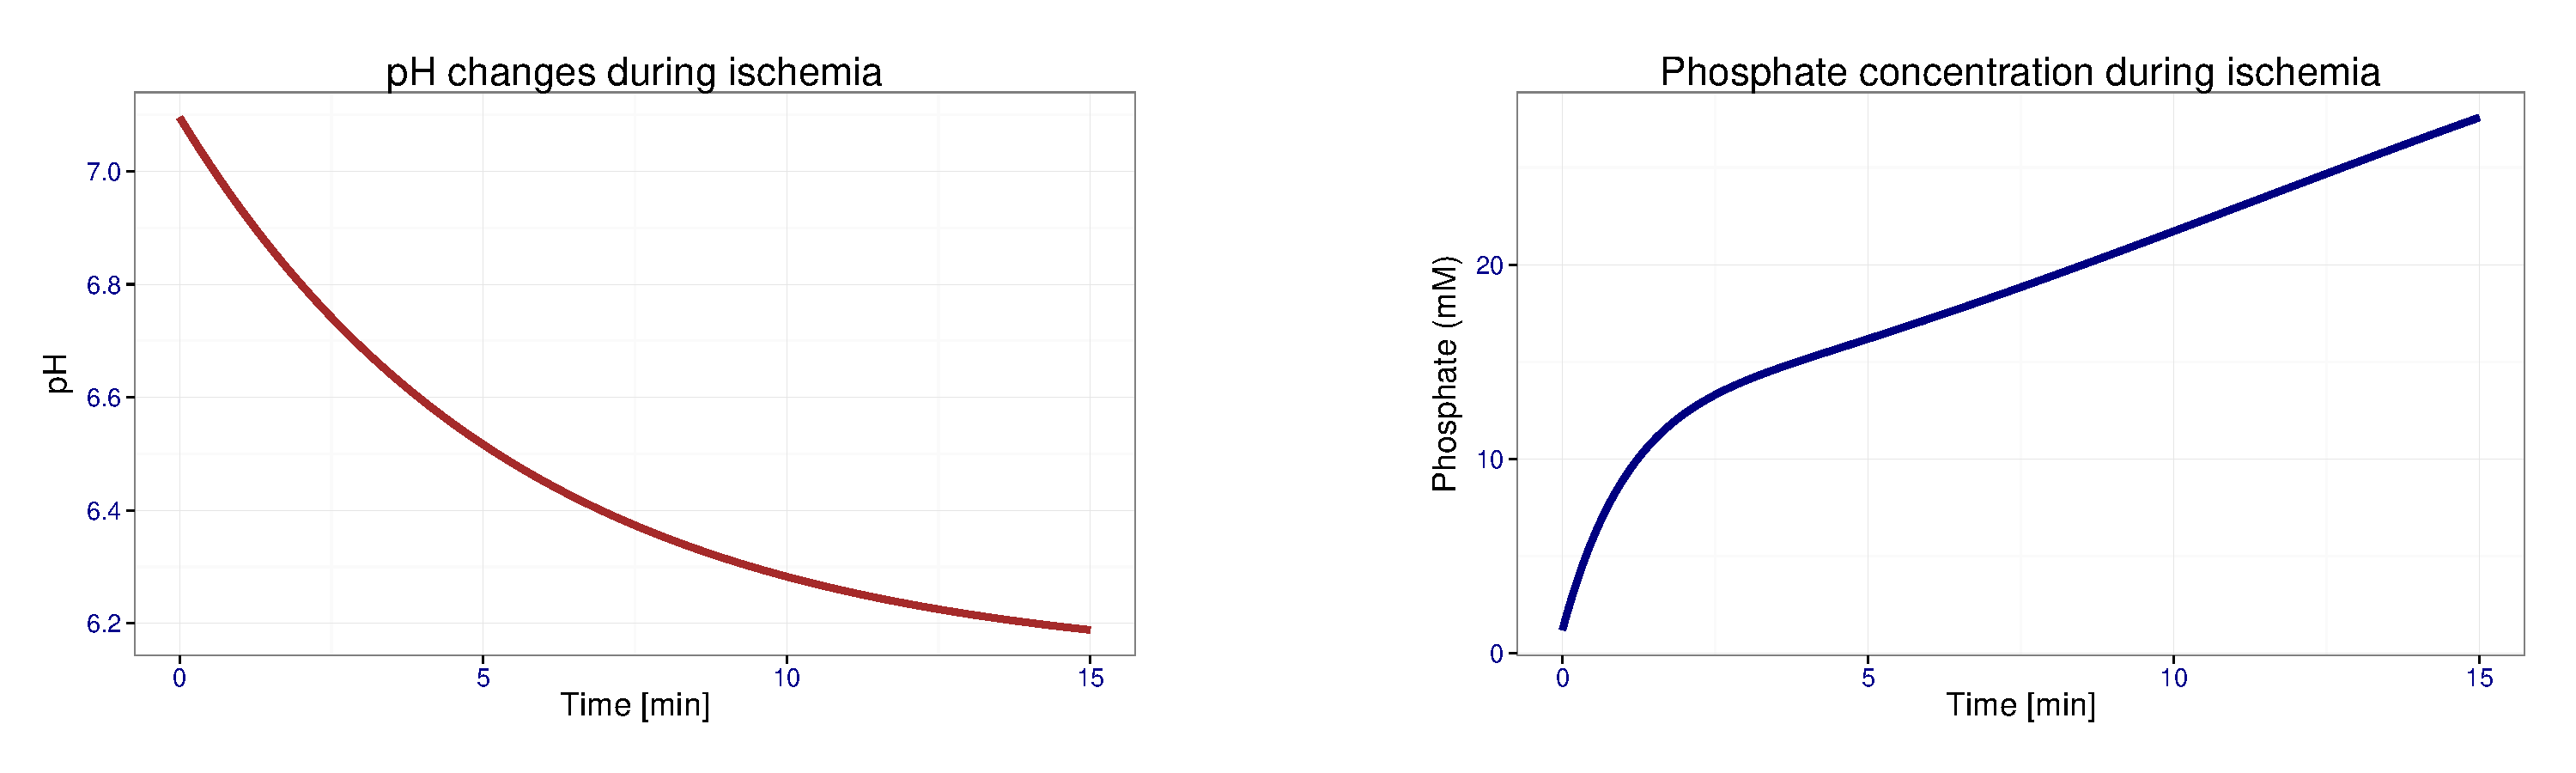
\includegraphics[scale=1.0]{poster/graf1}
\captionof{figure}{\color{Green} Figure caption}
\end{center}%\vspace{1cm}

\begin{center}%\vspace{1cm}
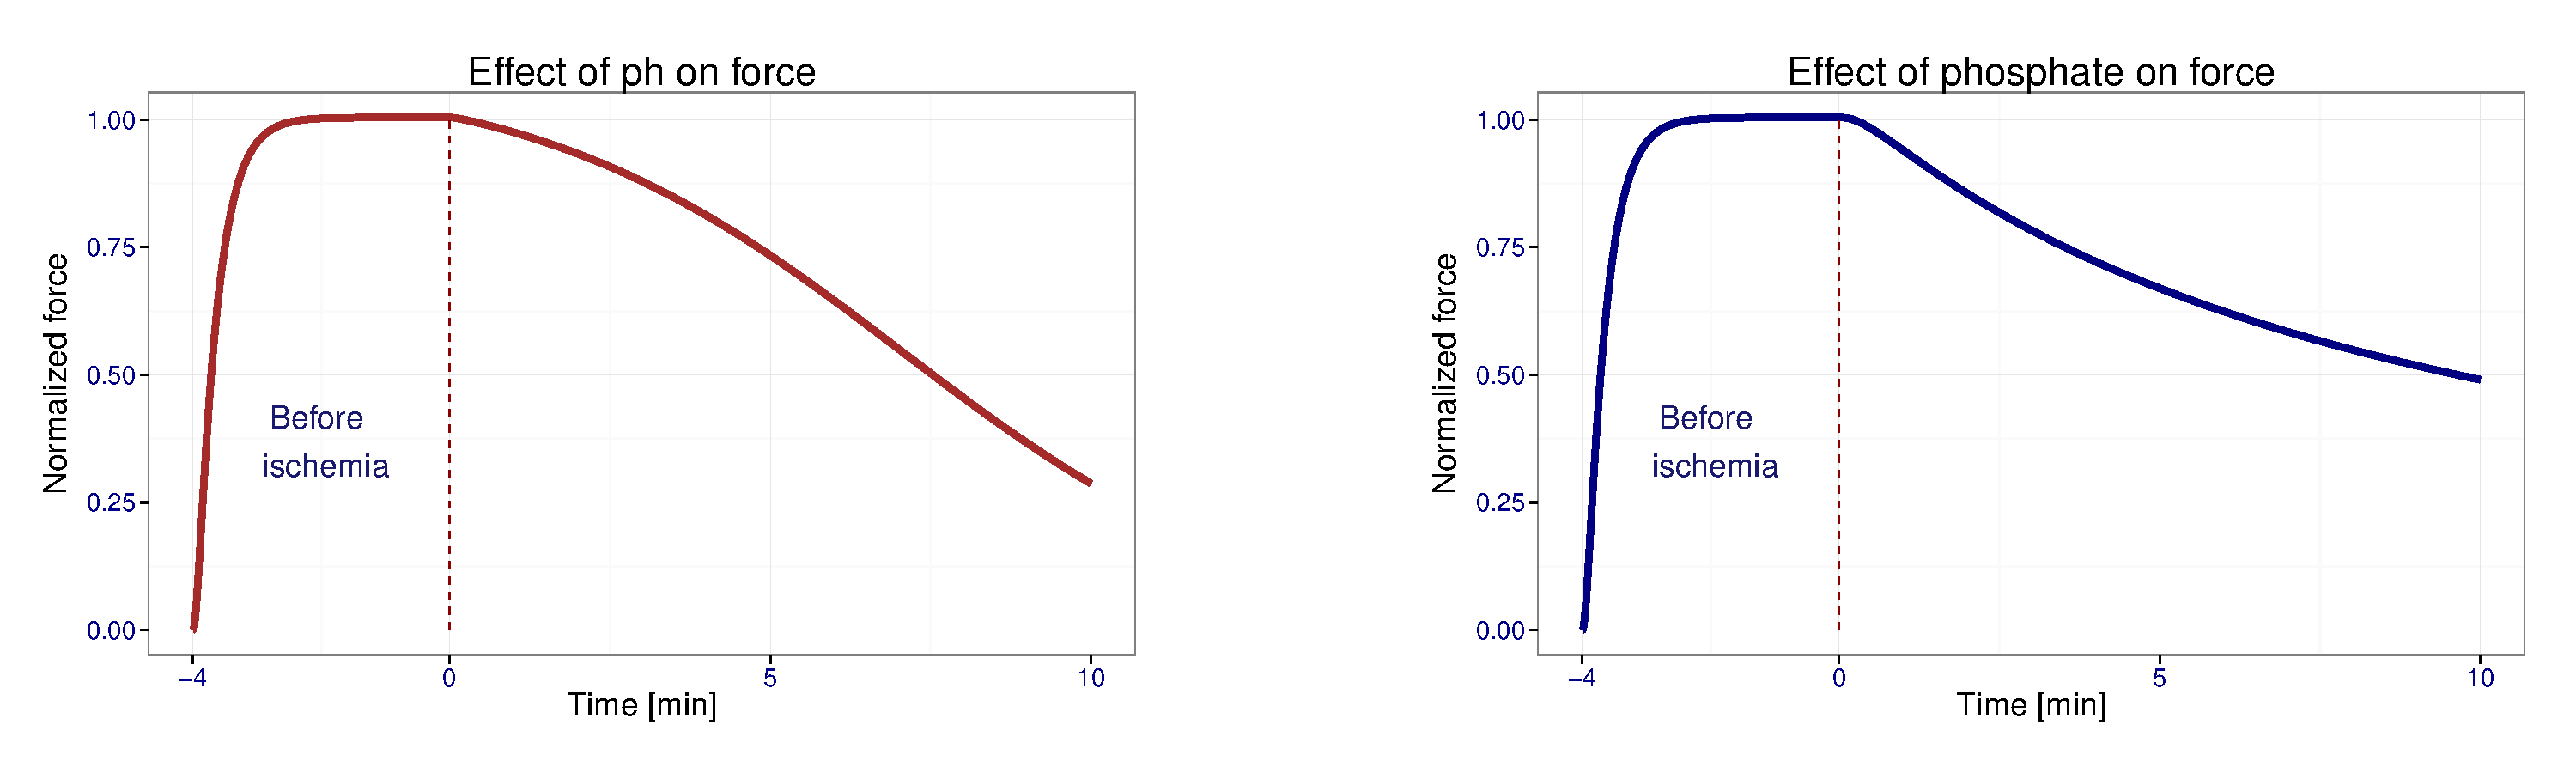
\includegraphics[scale=1.0]{poster/graf2}
\captionof{figure}{\color{Green} Figure caption}
\end{center}%\vspace{1cm}

Vivamus sed nibh ac metus tristique tristique a vitae ante. Sed lobortis
mi ut arcu fringilla et adipiscing ligula rutrum. Aenean turpis velit,
placerat eget tincidunt nec, ornare in nisl. In placerat.

\begin{center}%\vspace{1cm}
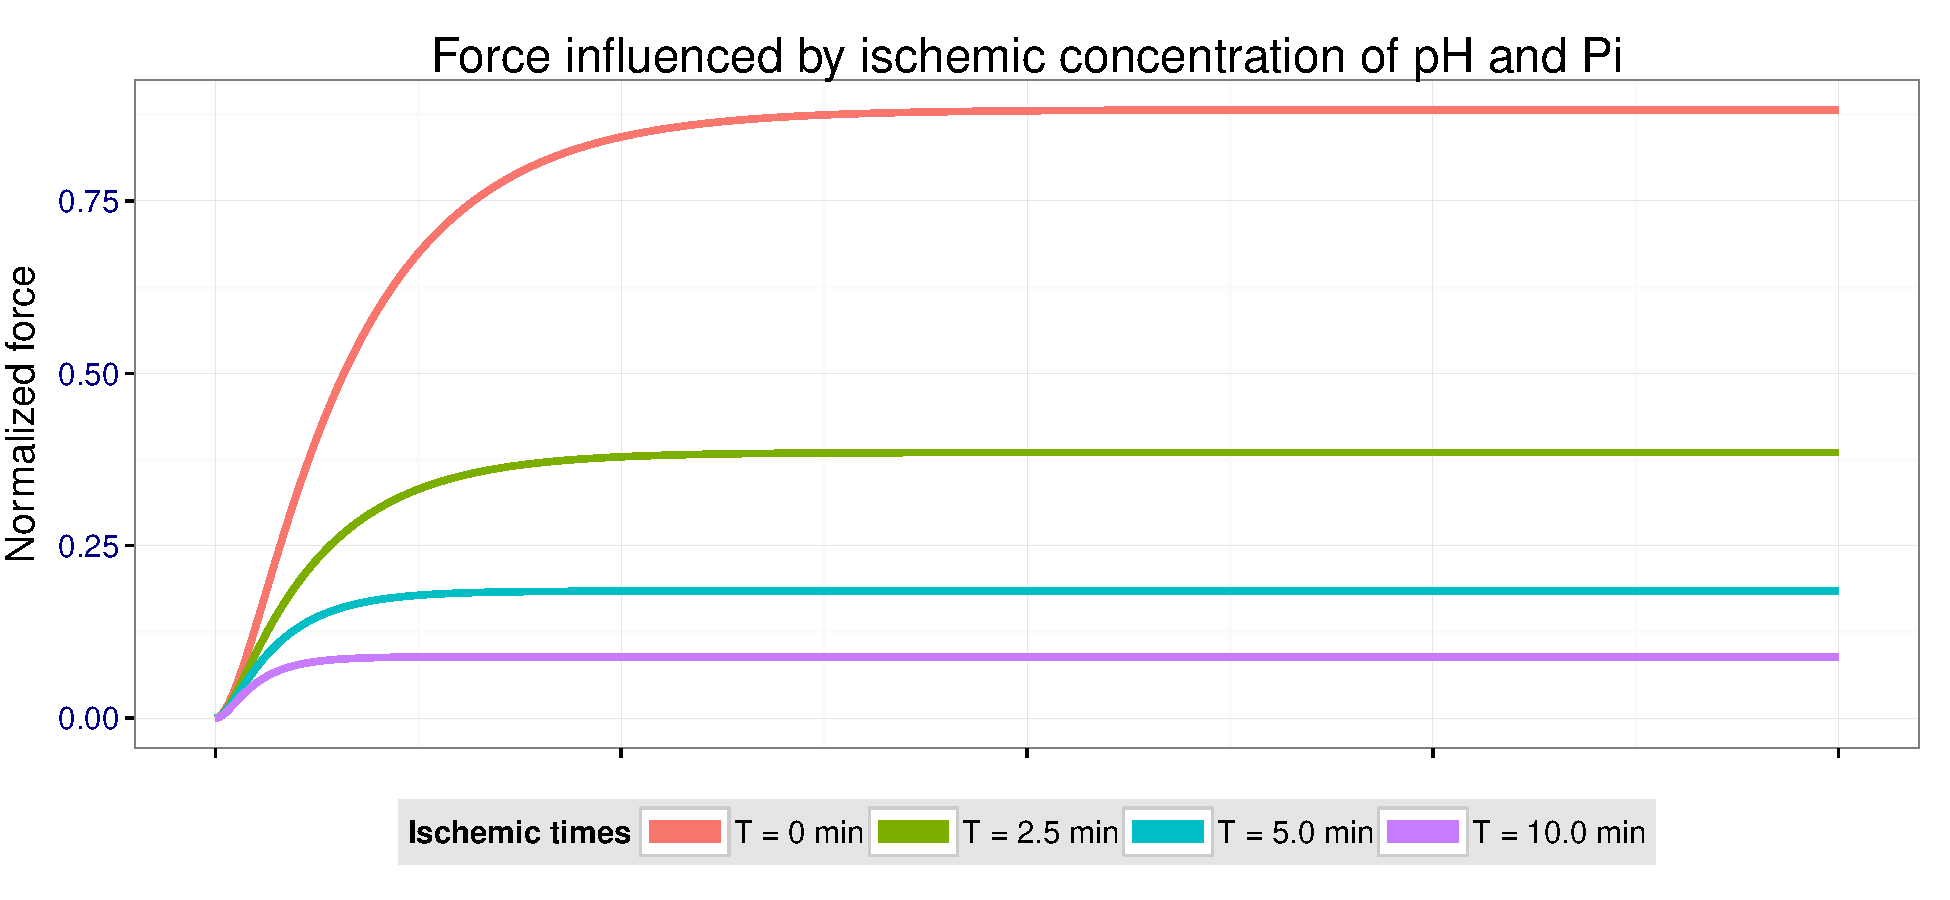
\includegraphics[scale=1.0]{poster/graf3}
\captionof{figure}{\color{Green} Figure caption}
\end{center}%\vspace{1cm}

%\begin{center}\vspace{1cm}
%\includegraphics[width=0.8\linewidth]{placeholder}
%\captionof{figure}{\color{Green} Figure caption}
%\end{center}\vspace{1cm}

%----------------------------------------------------------------------------------------
%   CONCLUSIONS
%----------------------------------------------------------------------------------------

\color{SaddleBrown} % SaddleBrown color for the conclusions to make them stand out

\section*{Conclusions}

\begin{itemize}

\item Pellentesque eget orci eros. Fusce ultricies, tellus et pellentesque
    fringilla, ante massa luctus libero, quis tristique purus urna nec
    nibh. Phasellus fermentum rutrum elementum. Nam quis justo lectus.
\item Vestibulum sem ante, hendrerit a gravida ac, blandit quis magna.
\item Donec sem metus, facilisis at condimentum eget, vehicula ut massa.
    Morbi consequat, diam sed convallis tincidunt, arcu nunc.
\item Nunc at convallis urna. isus ante. Pellentesque condimentum dui.
    Etiam sagittis purus non tellus tempor volutpat. Donec et dui non
    massa tristique adipiscing.
\end{itemize}

\color{DarkSlateGray} % Set the color back to DarkSlateGray for the rest of the content

%----------------------------------------------------------------------------------------
%   FORTHCOMING RESEARCH
%----------------------------------------------------------------------------------------

\section*{Forthcoming Research}

Vivamus molestie, risus tempor vehicula mattis, libero arcu volutpat
purus, sed blandit sem nibh eget turpis. Maecenas rutrum dui blandit lorem
vulputate gravida. Praesent venenatis mi vel lorem tempor at varius diam
sagittis. Nam eu leo id turpis interdum luctus a sed augue. Nam tellus.

 %----------------------------------------------------------------------------------------
%   REFERENCES
%----------------------------------------------------------------------------------------
\section*{References}

J. J. Rice, F. Wang, D. M. Bers, and P. de Tombe. \textit{Biophys J.}, \textbf{95(5):}2368-2390, 2008.\\
K. Tran, N. P. Smith, D. S. Loiselle, and E. J. Crampin. \textit{Biophys J.}, \textbf{98(2):}267-376, 2010.\\
J. R. Terkildsen, E. J. Crampin, et all. \textit{Am J Physiol Heart Circ Physiol}, \textbf{293(5):}H3036-H3045, 2007.

%\nocite{*} % Print all references regardless of whether they were cited in the poster or not
%\bibliographystyle{science} % Plain referencing style
%\bibliography{Heraeus_poster} % Use the example bibliography file sample.bib

%----------------------------------------------------------------------------------------
%   ACKNOWLEDGEMENTS
%----------------------------------------------------------------------------------------

\subsection*{Acknowledgements}

\small{Typesetting by {\LaTeX} using the \texttt{a0poster} class
created by Gerlinde~Kettl and Matthias~Weiser (\texttt{tex@kettl.de}).\\
Template from: \texttt{http://www.LaTeXTemplates.com} (License: CC BY-NC-SA 3.0)}

%----------------------------------------------------------------------------------------

\end{multicols}
\end{document}
